\chapter{Related Work}

TODO: Introduction for this section. 

\section{Reducing the burden of self tracking}
Self tracking can solve the problem of memory recall bias, by letting the user register observation in the moment (or very close to) they occur. But requiring the user to log observation introduces a burden of the work involved in doing so. As mention traditionally this has been done with pen and paper, but with the invention of smartphones and smartwatches this burden can be reduces. The work of Ponnada et al., 2017\cite{compare} investigate the interruption burden with both smartphones and smartwatches when used to with both regular EMA and $\mu$EMA. The difference between EMA and $\mu$EMA is that EMA will prompt the use less than $\mu$EMA, but requires the user to answer several questions back to back, where $\mu$EMA will instead prompt the user much more frequently, but only require the user to answer one question, which can be answered on the same screen showing the question. 

In a prior 4 week pilot study Ponnada et al. found that smartwatch $\mu$EMA demonstrated higher response rates and participants reported a lower perceived burden than smartphone EMA, even though the interruption rate for smartwatch $\mu$EMA was 8 times higher than smartphone EMA. In a new 4 week study they gathered data based on a smartwatch EMA in order to determine if the previous result where due to the fact that the data was gathered on a watch, or if it in fact was due to the $\mu$EMA. Their results showed that there were no statistically significant differences in compliance, completion, and first-prompt response rates observed between smartphone EMA and smartwatch EMA. But smartwatch $\mu$EMA response rates where significantly higher than smartwatch EMA. Their results suggest that the higher compliance and lower perceived burden is more likely to do with $\mu$EMA than the device itself and that compliance with EMA may not improve simply by changing the device.

The work of Ponnada et al. only looked into EMA where the device prompts the user for information, not situations where the user registers an observation. In his thesis Kami\'nski, 2016\cite{tomas} investigates how to enable self logging with different forms of input: a binary sample, selection input form a list, VAS and a numerical scale. He designed and implemented all of the input methods onto a smartwatch, where on the watch face each method input method could be selected. In figure \ref{tomas_design} we can see his design, the watch face has a shortcut for each input method. In figure \ref{tomas_design2} we see how the interaction occurs, and that it takes 1-3 touches to log the desired data depending on the input method.

\begin{figure}[h!]
    \centering
    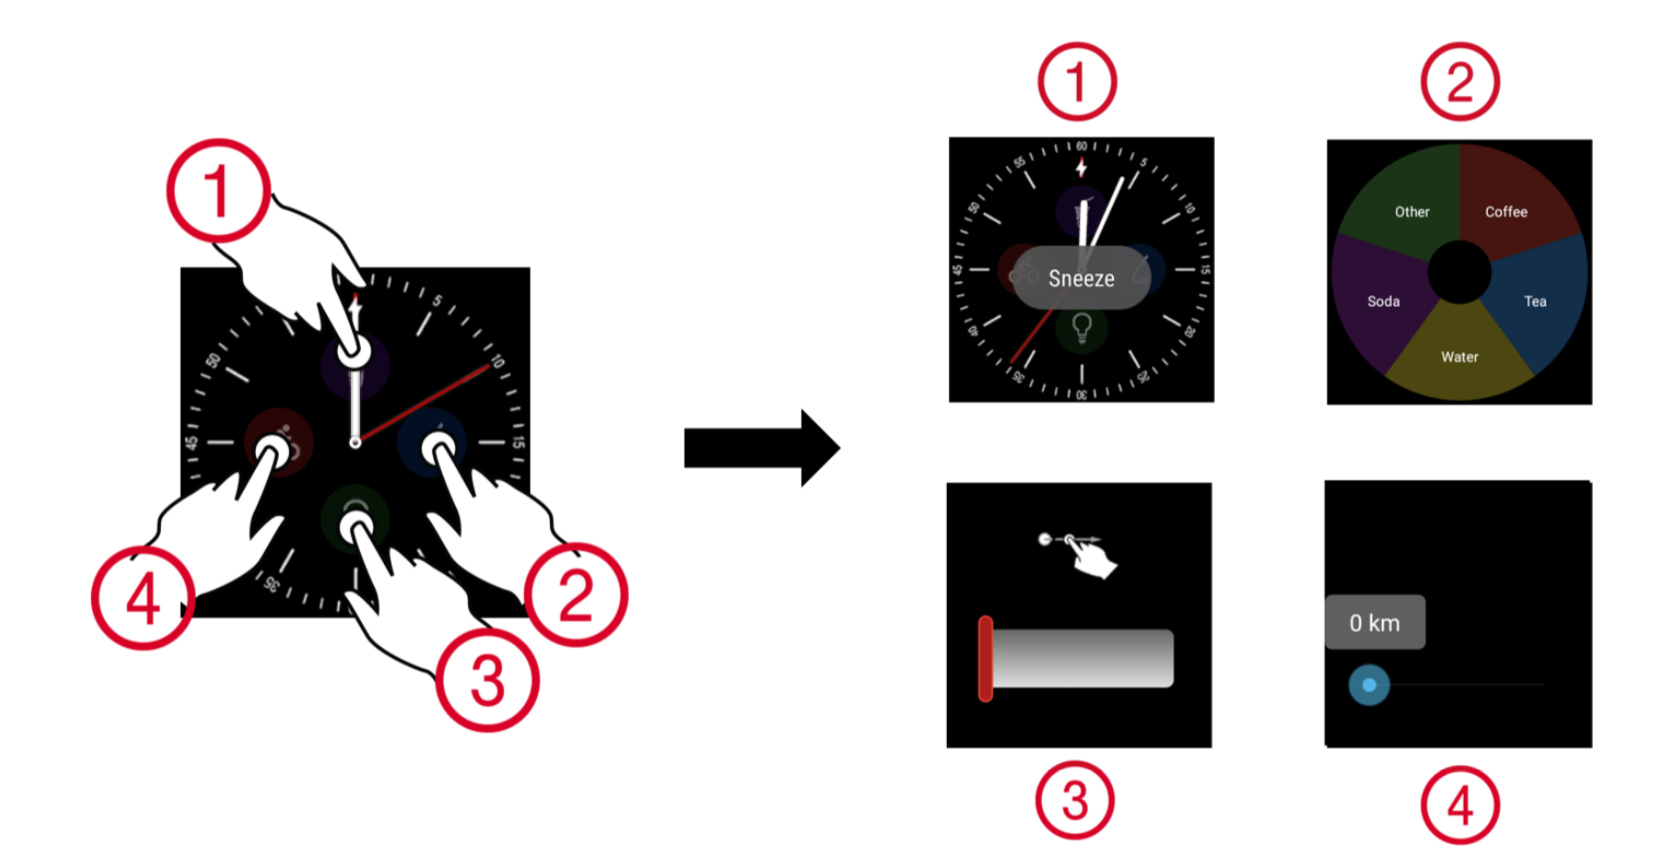
\includegraphics[width=1\textwidth]{figures/tomas_design.png}
    \caption{Design for self logging on a smartwatch by Kami\'nski\cite{tomas}}
    \label{tomas_design}
\end{figure}

\begin{figure}[h!]
    \centering
    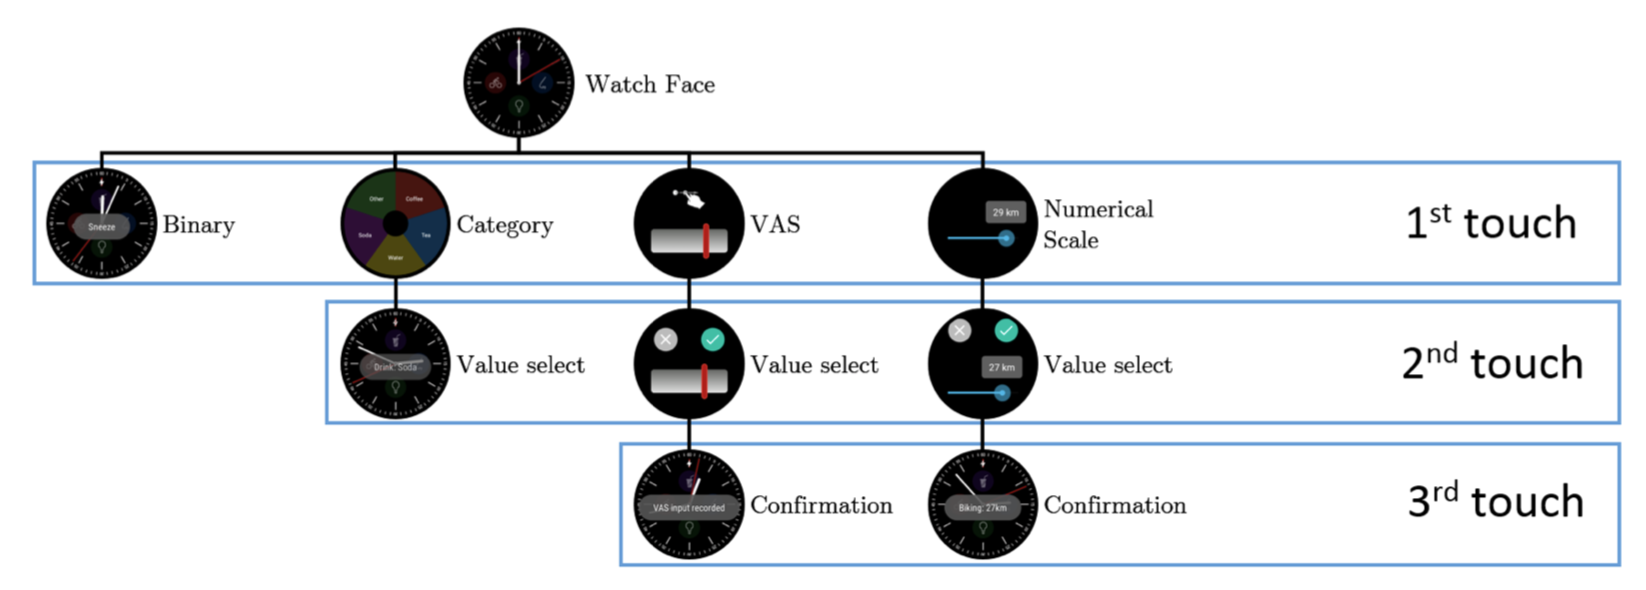
\includegraphics[width=1\textwidth]{figures/tomas_design2.png}
    \caption{Interaction for self logging on a smartwatch by Kami\'nski\cite{tomas}}
    \label{tomas_design2}
\end{figure}

For comparison Kami\'nski also implemented his a similar design on a smartphone following the \emph{Android material design guide}\cite{android_design} and conducted an experiment where he compared the two devices performance (interaction time, lower is better). His result showed a reduction in the user interaction time by approximately 30\% on average, thus successfully reducing the burden related to self logging. Beside his experiment Kami\'nski also had himself and to others use his design to collect data about their daily life (sneezing, skin itching and water consumption) over a 13-21 week period. What he found was a high compliance rate, all though it is a fairly biased test, since all three participants where involved in the project and are working with self logging technologies on a daily basis. 

Even though Kami\'nski design was a success, there persist an underlying problem with smartwatches; that they still require the user to user to activate them (often by tapping the screen or rotating their arm) and then the user has to look at the screen to touch the right section to register the input. Dam-Jensen, 2018\cite{dam} investigates this issue in his thesis. He introduces three ways of performing self logging, all using a \say{smartbutton} (wireless button connected to smartphone/smartwatch) to achieve a display-less logging system. The three input method that Dam-Jensen designed was:

\begin{enumerate}
	\item Hold Button: Measure the time the button is held down.
	\item Rotate Lower Arm: Using the built in gyroscope in the smartbutton, the difference in rotation from when the button was pressed to it was released is measured. In order to achieve a measurement the user would hold the button in the hand, rotate the lower arm to a neutral position, hold down the button, rotate the lower arm to the end position and release the button. 
	\item Rotate Upper Arm Around Elbow: Similar to the previous method, but instead of rotating the lower arm, the user would raise/lower his/hers upper arm around the elbow.
\end{enumerate}

For a comparison baseline method a standard VAS was used. In order to compare his three methods to the VAS Dam-Jensen conducted an experiment based on the work of Matejka et al., 2016 \cite{grey}, where participants are asked to rate a color between white and black on a grey scale where the colors are equally spaced out on the CIELAB color space\cite{cielab} (more on this later). His results showed that there where no significant difference in accuracy between his three designed input methods compared and the baseline, thus meaning that all three methods are viable and could be used for self logging, and in their simple nature can reduce the burden on the user.

\section{Long term use of self logging}
As mentioned Ponnada et al. conducted two 4 weeks studies with EMA and $\mu$EMA and Kami\'nski conducted a even longer 13-21 week use case where three people used his design to track daily activities. Both Ponnada et al. and Kami\'nski work show great potential for real use, but none of them has been proper tested in the real world, also none of them utilizes a device similar to that of Dam-Jensen's work, where there is no screen and only a single button for registering observations.

In a case study Larsen et al., 2017\cite{eg} investigated the real life use case of a novel device for self logging. They had a Danish veteran suffering from post-traumatic stress disorder equipped with a \say{smartbutton}, that when pressed will store a time stamp. By connecting a smartphone the data can be transferred from the smartbutton to a data file for further analysis. The veteran was then instructed to press the button whenever he experienced a specific event related to his PTDS (the \say{trigger event} was chosen based on a two-hour assessment interview together with his therapist). The veteran wore smartbutton for 100, pressing the button whenever he experienced the specific event.

The results showed that the veteran had a high compliance, actively using the device throughout the 100 days (due to a technical issue no data was collected during the second week). The data collected revealed patterns that explained why/when the veteran's events would be triggered, which would not have revealed itself from the conversational assessment. In other words, not only was it a success from a technical and usability standpoint, but it also succeeded in bringing valuable new information to the treatment process. 

\section{Comparing ratings of behavior}
When developing new methods for self logging it is important to access the feasibility of these methods. As mentioned Kami\'nski did this simply by comparing the user interaction time, while Dam-Jensen did a more comprehensive comparison by looking into how precise the data recorded with his designs compared to the VAS. He did by having his participants rate shades of grey with the different input methods. That experiment was inspired by the work of Matejka et al., 2016 \cite{grey} where they investigate the bias of different slider designs. In order to do so they base their experiment on the work of Borg and Borg, 1991\cite{borg} that extensively studied using a \say{scale of blackness} as a stimulus and concluded that it serves as a good test of general rating behaviour, and further more it provides a truth value (the color displayed) with can be compared to the response rating from the participant. Matejka et al. designed their experiment to test severely different slider designs with various combinations of labels, tick marks and bands. In figure \ref{mate_ex} a design with 2 labels and 5 ticks is shown. Matejka et al. recruited participants via \emph{Amazon Mechanical Turk}\cite{turk}. Participants where then showed one of the 50 shades of grey (as seen in figure \ref{50shades}), then asked to rate the color from white to blakc using the slider. This process was repeated several 50 times so each participants was exposed to all the shades of grey (in random order), this was then repeated until the participants had been exposed to each shade of grey 4 times, 200 trials in total. Each participant was only exposed to one slider design, and was afterwards excluded to participate further. 

\begin{figure}[h!]
    \centering
    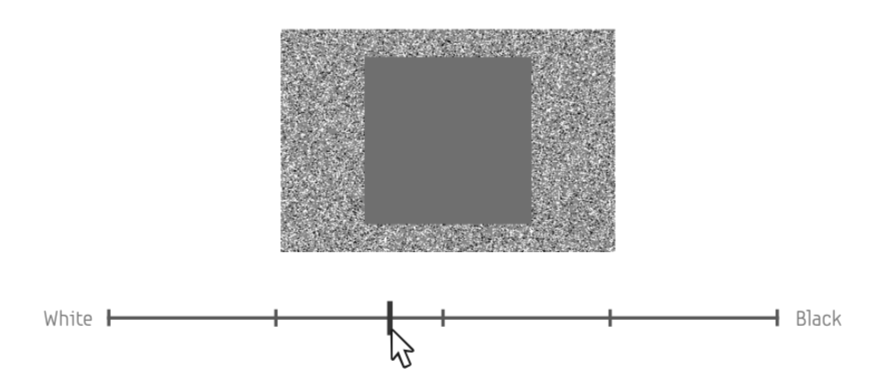
\includegraphics[width=1\textwidth]{figures/mate_ex.png}
    \caption{Slider bias experiment by Matejka et al.\cite{grey} with 2 labels and 5 ticks}
    \label{mate_ex}
\end{figure}

\begin{figure}[h!]
    \centering
    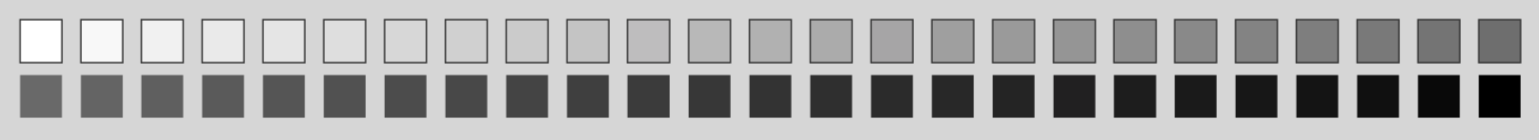
\includegraphics[width=1\textwidth]{figures/50shades.png}
    \caption{50 shades of grey used by Matejka et al.\cite{grey}}
    \label{50shades}
\end{figure}

With their results they investigated the bias for each slider design by looking at the distribution of responses and calculating a \say{smoothness} value representing the bias as well as precision and response time. Their results showed that sliders with ticks introduces the most bias towards the tick marks, followed by sliders with many labels and combination of the two. Banded sliders showed only small amount of bias and sliders with only two labels showed the least amount of bias. The higher amount of both ticks and labels resulted in higher precision.

\section{Relation to this thesis}
The work of Ponnada et al., Kami\'nski and Dam-Jensen all point towards the benefit reducing the burdens and show. Their work has been a great inspiration for this thesis, together with Larsen et al. work showing the real world benefit of in situ measurements. This thesis will further investigate two of Dam-Jensen's designs, the \say{Rotate Lower Arm} and \say{Rotate Upper Arm Around Elbow} methods together with the \say{rating of blackness} will be the starting point.